\documentclass[]{article}
\usepackage{lmodern}
\usepackage{amssymb,amsmath}
\usepackage{ifxetex,ifluatex}
\usepackage{fixltx2e} % provides \textsubscript
\ifnum 0\ifxetex 1\fi\ifluatex 1\fi=0 % if pdftex
  \usepackage[T1]{fontenc}
  \usepackage[utf8]{inputenc}
\else % if luatex or xelatex
  \ifxetex
    \usepackage{mathspec}
    \usepackage{xltxtra,xunicode}
  \else
    \usepackage{fontspec}
  \fi
  \defaultfontfeatures{Mapping=tex-text,Scale=MatchLowercase}
  \newcommand{\euro}{€}
\fi
% use upquote if available, for straight quotes in verbatim environments
\IfFileExists{upquote.sty}{\usepackage{upquote}}{}
% use microtype if available
\IfFileExists{microtype.sty}{%
\usepackage{microtype}
\UseMicrotypeSet[protrusion]{basicmath} % disable protrusion for tt fonts
}{}
\usepackage[margin=1in]{geometry}
\ifxetex
  \usepackage[setpagesize=false, % page size defined by xetex
              unicode=false, % unicode breaks when used with xetex
              xetex]{hyperref}
\else
  \usepackage[unicode=true]{hyperref}
\fi
\hypersetup{breaklinks=true,
            bookmarks=true,
            pdfauthor={Jan Winter},
            pdftitle={caRpools Shortcut User Guide},
            colorlinks=true,
            citecolor=blue,
            urlcolor=blue,
            linkcolor=magenta,
            pdfborder={0 0 0}}
\urlstyle{same}  % don't use monospace font for urls
\usepackage{graphicx,grffile}
\makeatletter
\def\maxwidth{\ifdim\Gin@nat@width>\linewidth\linewidth\else\Gin@nat@width\fi}
\def\maxheight{\ifdim\Gin@nat@height>\textheight\textheight\else\Gin@nat@height\fi}
\makeatother
% Scale images if necessary, so that they will not overflow the page
% margins by default, and it is still possible to overwrite the defaults
% using explicit options in \includegraphics[width, height, ...]{}
\setkeys{Gin}{width=\maxwidth,height=\maxheight,keepaspectratio}
\setlength{\parindent}{0pt}
\setlength{\parskip}{6pt plus 2pt minus 1pt}
\setlength{\emergencystretch}{3em}  % prevent overfull lines
\providecommand{\tightlist}{%
  \setlength{\itemsep}{0pt}\setlength{\parskip}{0pt}}
\setcounter{secnumdepth}{5}

%%% Use protect on footnotes to avoid problems with footnotes in titles
\let\rmarkdownfootnote\footnote%
\def\footnote{\protect\rmarkdownfootnote}

%%% Change title format to be more compact
\usepackage{titling}

% Create subtitle command for use in maketitle
\newcommand{\subtitle}[1]{
  \posttitle{
    \begin{center}\large#1\end{center}
    }
}

\setlength{\droptitle}{-2em}
  \title{caRpools Shortcut User Guide}
  \pretitle{\vspace{\droptitle}\centering\huge}
  \posttitle{\par}
  \author{Jan Winter}
  \preauthor{\centering\large\emph}
  \postauthor{\par}
  \date{}
  \predate{}\postdate{}


% Redefines (sub)paragraphs to behave more like sections
\ifx\paragraph\undefined\else
\let\oldparagraph\paragraph
\renewcommand{\paragraph}[1]{\oldparagraph{#1}\mbox{}}
\fi
\ifx\subparagraph\undefined\else
\let\oldsubparagraph\subparagraph
\renewcommand{\subparagraph}[1]{\oldsubparagraph{#1}\mbox{}}
\fi

\begin{document}
\maketitle

{
\hypersetup{linkcolor=black}
\setcounter{tocdepth}{2}
\tableofcontents
}
\newpage

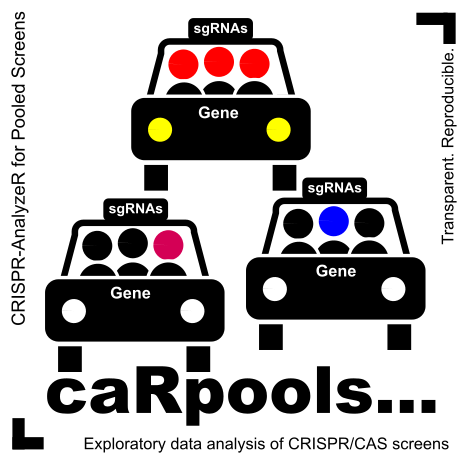
\includegraphics{./pictures/CaRpools.png}

\newpage

\section{Files and Folder Structure to use
CaRpools}\label{files-and-folder-structure-to-use-carpools}

\textbf{Please note: the MAIN FOLDER must be the R working directory!}\\
Data and Script paths can be adjusted in the MIACCS file.

The following files are neccessary to use CaRpools for report
generation:

\textbf{MIACCS.xls}\\
Minimum Information About CRISPR/Cas Screens. This file needs to be
filled out to provide all necessary informations about the screen.

\textbf{R Markdown Template files}\\
Either CaRpools-extended-PDF.rmd, CaRpools-PDF.rmd or
CaRpools-extended-HTML.rmd or CaRpools-HTML.rmd. Is the template for
report generation.

\textbf{Data Files}\\
Two replicates per Control and Treated. Can be FASTQ files OR already
mapped, not normalized read count files.

\textbf{CRISPR-mapping.pl}\\
PERL script to map your extracted FASTQ files, if desired (as indicated
in the MIACCS.xls)

\textbf{CRISPR-extract.pl}\\
PERL script to extract 20 nt target sequence from FAST files, if desired
(as indicated in the MIACCS.xls)

\textbf{CaRpools.png}\\
The logo file

The following files are necessary to use \emph{single} CaRpools
functions:

\textbf{Data Files}\\
Either raw read count files or FASTQ files (that need to be extracted
and mapped using CaRpools)

Please note that CaRpools always starts with loading data files. For
raw-readcount files, use \texttt{load.file}. For FASTQ files, please see
the sections below.

\textbf{CaRpools folder structure for Report Generation using raw Read
Count files:}

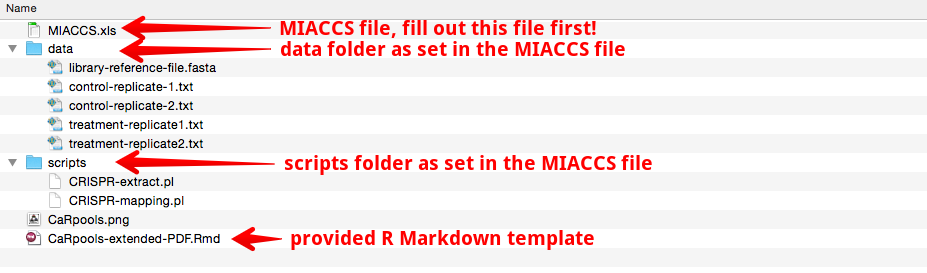
\includegraphics{./pictures/folder-structure-before.png}

\textbf{CaRpools folder structure for Report Generation using raw Read
Count files AFTER REPORT GENERATION:}

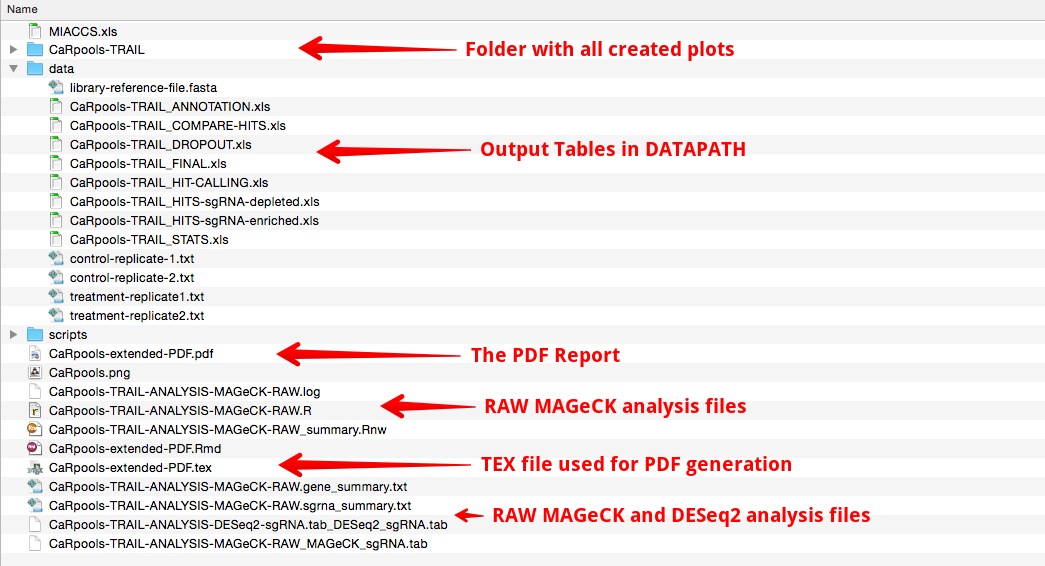
\includegraphics{./pictures/folder-structure-FINAL.png}

\textbf{CaRpools folder structrue for Report Generation using FASTQ
files:}

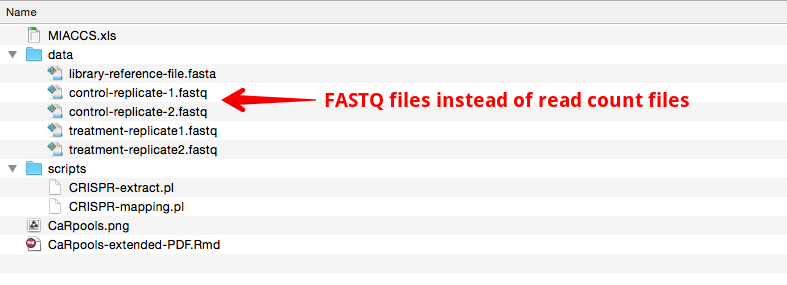
\includegraphics{./pictures/folder-structure-FASTQ-before.png}

\textbf{CaRpools folder structure for Report Generation using FASTQ
files AFTER REPORT GENERATION:}

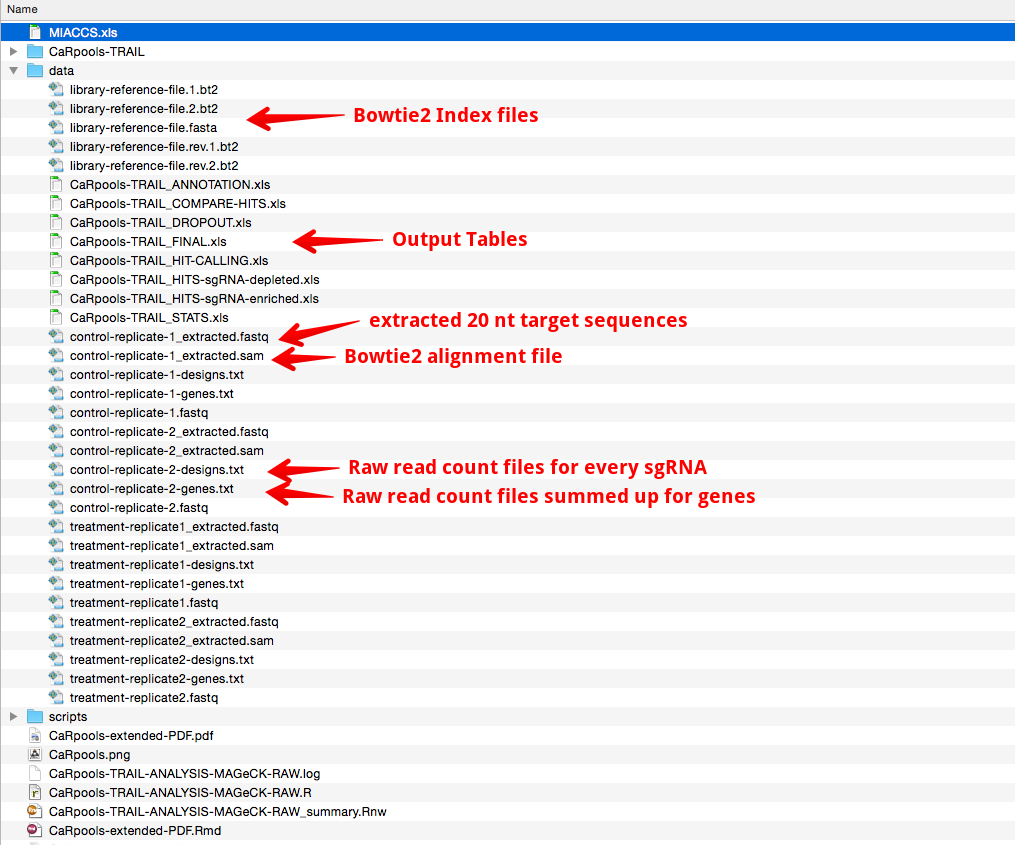
\includegraphics{./pictures/folder-structure-FASTQ-FINAL.png}

\newpage

\subsection{Start CaRpools VirtualBox
Image}\label{start-carpools-virtualbox-image}

\textbf{Please see }CaRpools-SHORTGUIDE-VirtualBox.pdf/html** or the
shortguid
\href{https://github.com/boutroslab/caRpools/blob/master/docs/CaRpools-SHORTGUIDE-VirtualBox.Rmd}{here}
for how to use it.

\subsection{Setup Files and R-Studio on your own
computer}\label{setup-files-and-r-studio-on-your-own-computer}

All packages and software tools need be installed correctly as shown
before.

\begin{enumerate}
\def\labelenumi{\arabic{enumi}.}
\tightlist
\item
  Copy all files in the designated folders as shown above.
\end{enumerate}

\begin{itemize}
\tightlist
\item
  \textbf{Please note: the MAIN FOLDER must be R working directory!}
\item
  The MIACCS.xls as well the R markdown template and CaRpools.png must
  be in the same folder as the R working dir.
\end{itemize}

\begin{enumerate}
\def\labelenumi{\arabic{enumi}.}
\setcounter{enumi}{1}
\tightlist
\item
  Adjust the path to the data and scripts folder if necessary in the
  MIACCS.xls . Use the absolute path. If the folder structure is as
  shown above, you do not need to make any adjustments.
\item
  Adjust and fill out the \textbf{MIACCS.xls} file.
\item
  You can use \texttt{CarPools(type="check")} to check for the correct
  folder structure and data file presence as it is indicated in the
  MIACCS.xls file.
\item
  You can check for your R working directory by \texttt{getwd()} and set
  it to any directory you want by \texttt{setwd("/PATH")}.
\end{enumerate}

\subsection{Check Setup}\label{check-setup}

You can verify that the MIACCS.xls file as well as the used template
file and all necessary scripts are found by calling
\texttt{check.caRpools()}.\\
See below for more information about the arguments.\\
By default, it \textbf{requires a correct MIACCS file + the script files
+ all packages installed + MAGeCK + Bowtie2 + Pandoc.}

\subsection{Example of a MIACCS File entry for FASTQ
files}\label{example-of-a-miaccs-file-entry-for-fastq-files}

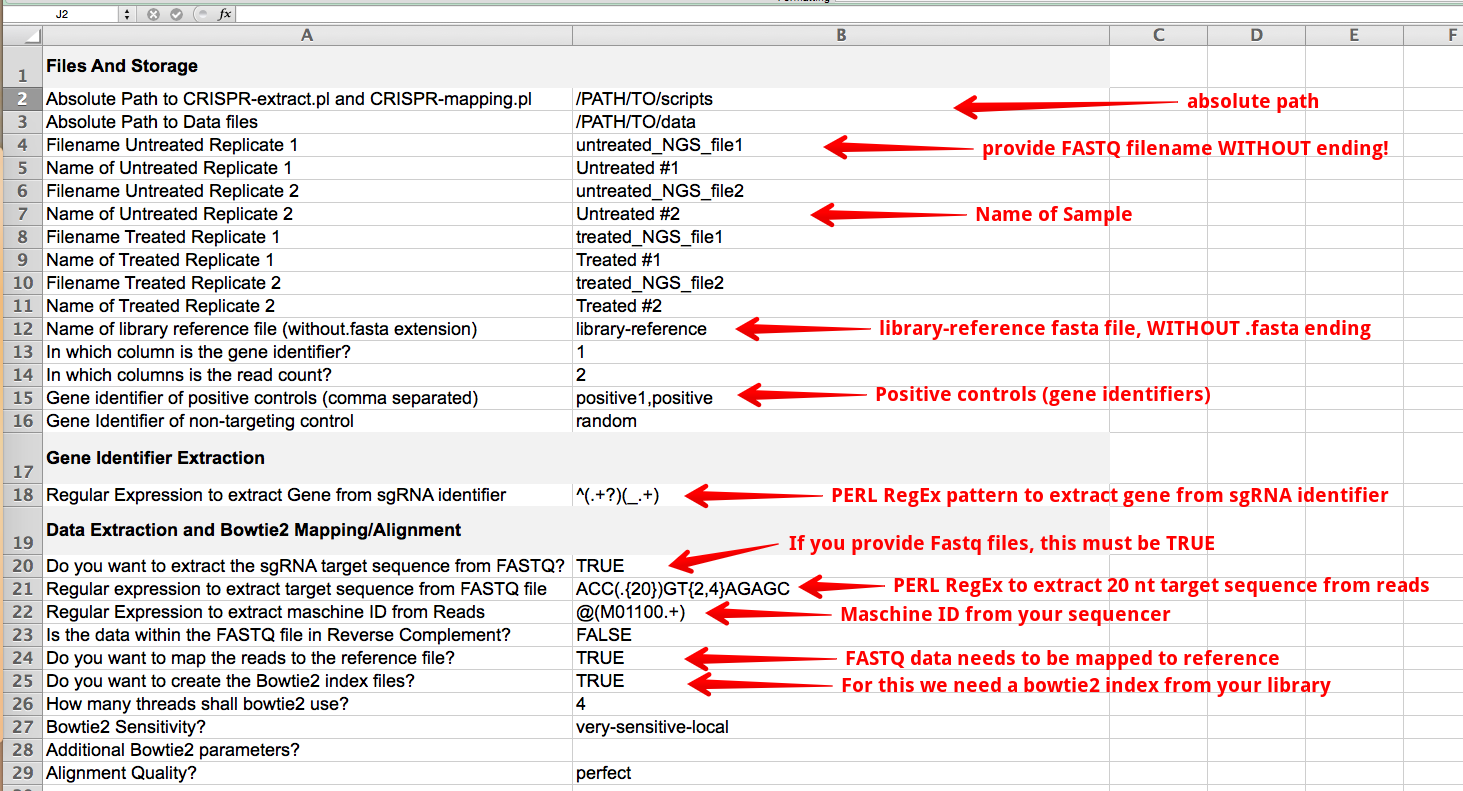
\includegraphics{./pictures/miaccs-fastq.png}

\subsection{Example of a MIACCS File entry for Read-Count
files}\label{example-of-a-miaccs-file-entry-for-read-count-files}

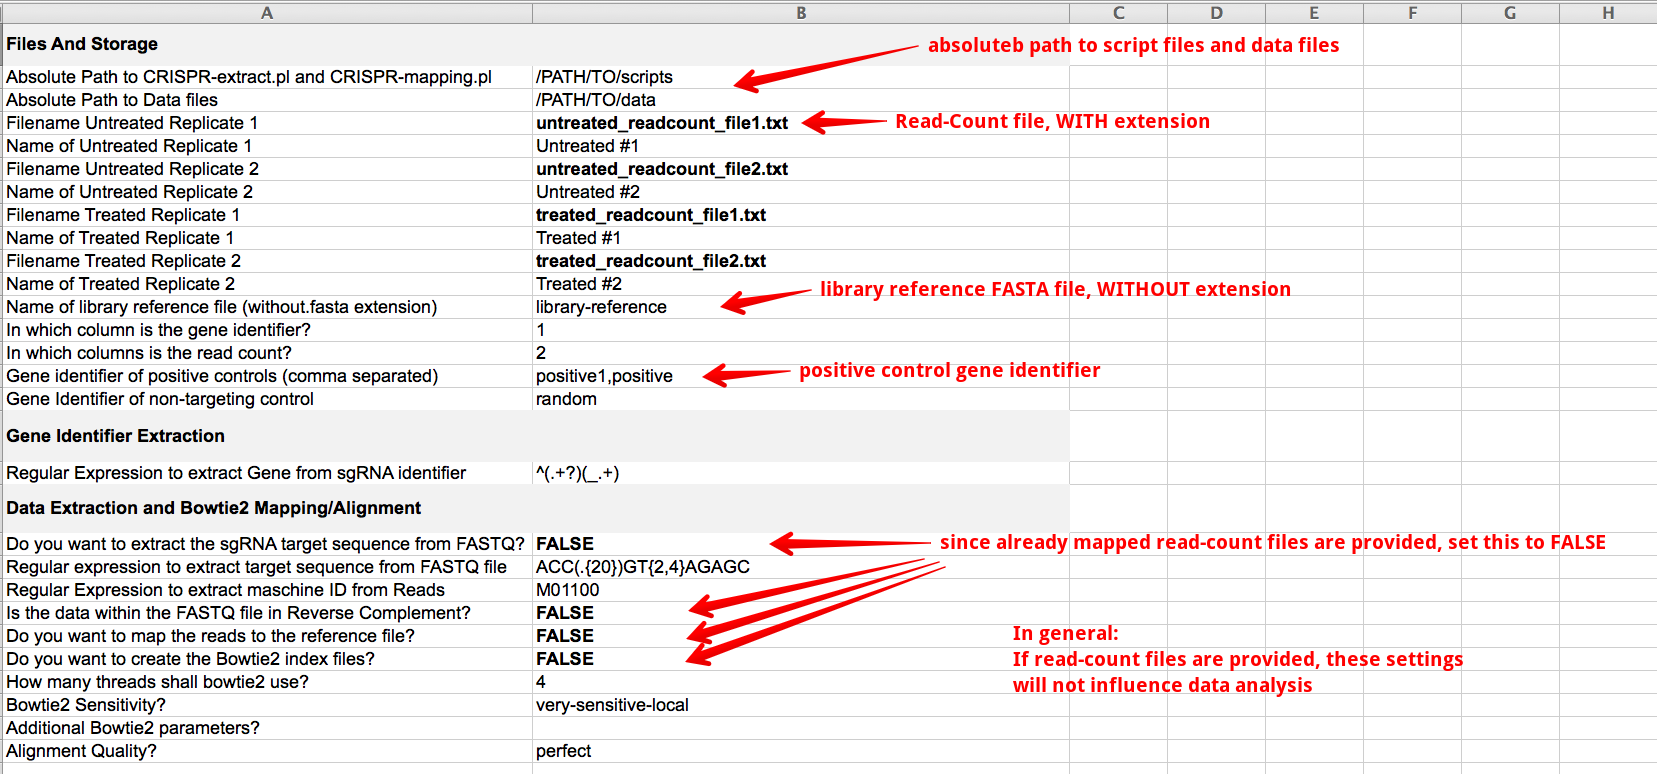
\includegraphics{./pictures/miaccs-readcount.png}

\section{Start CaRpools Report
Generation}\label{start-carpools-report-generation}

You can start caRpools Report Generation after you did the following
steps:

\begin{itemize}
\tightlist
\item
  Installed all required software and R packages (use
  \emph{check.caRpools(files=FALSE)} to verify)
\item
  Put every file in the correct folder (MIACCS, data files, script
  files, Rmd templates)
\item
  Put everythin in the R working directory or set the working directory
  to the folder of your files
\item
  Filled out the MIACCS file with all information, e.g.~correct
  filenames, reference, data analysis options
\end{itemize}

You can check for all requirements by calling \texttt{check.caRpools}.

\subsection{Start CaRpools using
R-Studio}\label{start-carpools-using-r-studio}

In the case you use R-Studio, you can start caRpools by just opening the
corresponding Rmd template file.\\
At the top, you will find the \textbf{Knit PDF} or \textbf{Knit HTML}
button, so you just need to press that and caRpools will generate the
report.

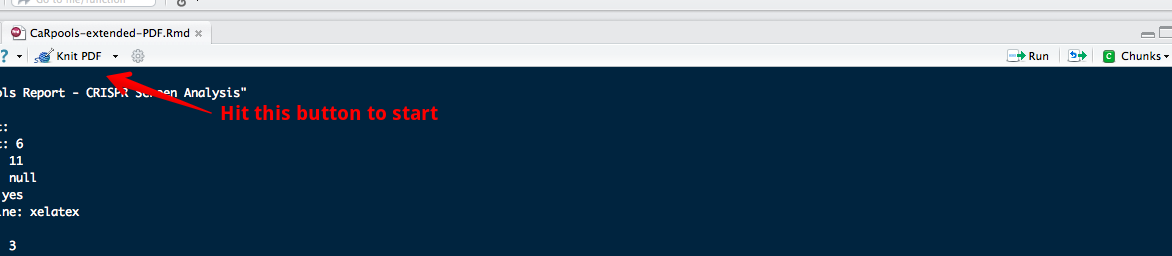
\includegraphics{./pictures/rstudio-knit.png}

As an alternative, you can start caRpools via \texttt{use.caRpools} and
provide additional parameters (see below).

\subsection{Start CaRpools using R
console}\label{start-carpools-using-r-console}

Moreover, caRpools report generation can also be initiated without
R-studio installation, so that this can be done via R command line even
on remote computers.\\
In this case, caRpools report generation can be started via
\texttt{use.caRpools} with additional parameters, which are described
below.

\paragraph{use.caRpools()}\label{use.carpools}

\textbf{Usage:}\\
\emph{use.caRpools(type=NULL, file=``CaRpools-extended-PDF.Rmd'',
miaccs=``MIACCS.xls'', check=TRUE, work.dir=NULL)}

\textbf{type}\\
\emph{Description} If you provide a custom Rmd template that can
generate both, PDF and HTML reports you can indicate which version you
want to generate.\\
\emph{Default} NULL\\
\emph{Values} ``PDF'', ``HTML''

\textbf{file}\\
\emph{Description} The file name of your custom Rmd template file (with
extension).\\
\emph{Default} ``CaRpools-extended-PDF.Rmd''\\
\emph{Values} filename as character

\textbf{miaccs}\\
\emph{Description} The filename of your MIACCS file.\\
\emph{Default} ``MIACCS.xls''\\
\emph{Values} filename as character

\textbf{check}\\
\emph{Description} Indicates whether caRpools will check for correct
installation and file access.\\
\emph{Default} TRUE\\
\emph{Values} TRUE or FALSE (boolean)

\textbf{work.dir}\\
\emph{Description} You can provide the absolute path to the working
directory in which all files are placed (e.g.~the MIACCS.xls and Rmd
template).\\
\emph{Default} NULL \emph{Values} absolute path (character) or NULL if
standard R working directory is used

\end{document}
